\documentclass{beamer}

\usepackage{biblatex}
\usepackage{bookmark}
\usepackage[czech]{babel}
\usepackage{csquotes}

\usetheme{Berkeley}
\addbibresource{../bakalarka.bib}
\addbibresource{prezentace.bib}

\author{Matěj Sloup}
\date{11. 12. 2025}
\title{Bakalářská práce}
\subtitle{Modelování cen finančních aktiv diskrétními Markovskými řetezci a jejich aplikace v opčních strategiích}

\begin{document}

\begin{frame}
  \titlepage
\end{frame}

\section{Obsah prezentace}
\begin{frame}{Obsah}
  \tableofcontents
\end{frame}

\section{Rámec práce}
\begin{frame}{Cíl práce}
  \begin{itemize}
    \item{Model markovského řetezece pro vývoj ceny akcie}
      \begin{itemize}
        \item{Použito pro předpověď ceny akcie a spjaté opce}
      \end{itemize}
    \item{Webová aplikace pro vizualizaci předpovědi}
      \begin{itemize}
        \item{Graf hodnoty odhadovaného vývoje x reálná hodnota}
        \item{Analýza opce (volatilita, hodnota, apod.)}
        \item{Doporučená strategie}
      \end{itemize}
  \end{itemize}
\end{frame}

\section{Úvod do problematiky}

\subsection{Markovské řetezce}

\begin{frame}{Náhodný proces}
  \begin{block}{Náhodný proces}
    Náhodný proces definujeme jako množinu náhodných veličin, závislých na určitém počtu parametrů náležících množině reálných čísel. \cite{korenar2010}
  \end{block}

  \begin{block}{Stochastický proces}
    Je-li jediným parametrem náhodného procesu čas, označujeme takovýto proces jako stochastický. \cite{korenar2010}
  \end{block}

  Stochastický proces značíme kupříkladu $X(t)$, kde $X$ je náhodný proces, a $t$ je parametr náležicí množině parametrů $T$ (u stochastických procesů množina časových okamžiků). \cite{korenar2010}
\end{frame}

\begin{frame}{Markovská podmínka}
  \begin{block}{Matematická formulace}
    Nechť $X(t); t \in \{1,2, ... , n\}$ je stochastický proces, a nechť $s(t) = j$ značí stav procesu v momentu $t$ náležící množině stavů. Pro tento proces platí Markovská podmínka právě tehdy, když:
    \begin{multline*}
      P(s(t) = j_1 | s(t-1) = j_2, s(t-2) = j_3, ... , s(1) = j_n) \\
      = P(s(t) = j_1 | s(t-1) = j_2)
    \end{multline*}
    \cite{lukas2009}
  \end{block}

  Stochastický proces splňující Markovskou podmínku nadále budeme nazývat Markovským procesem.
\end{frame}

\begin{frame}{Markovský řetezec}
  \begin{block}{Markovský řetezec}
    Markovský řetezec je Markovský proces s diskrétní množinou parametrů a diskrétní množinou stavů. \cite{lukas2009}
  \end{block}

  %TODO: Vymysli něco lepšího.
  Rozeznáváme různé typy řetezců:
  \begin{itemize}
    \item{Tranzientní x rekurentní}
    \item{Absorpční}
    \item{Regulérní}
  \end{itemize}
\end{frame}

\subsection{Opce}

\begin{frame}{Opce}
  \begin{block}{Definice}
    Opce jsou finanční kontrakt, který dává kupujícímu právo koupit/prodat v budoucnosti od prodávajícího nějaký podkladové aktivum za předem dohodnutou (strike) cenu. \cite{plechac2021}
  \end{block}

  \begin{itemize}
    \item Derivát
    \item Prémie
  \end{itemize}
\end{frame}

\begin{frame}{Obchodování s opcemi}
  \begin{itemize}
    \item Call opce x Put opce
    \item Short pozice x Long pozice
      \begin{itemize}
        \item Kupující a vypisující %TODO: ROZVEĎ MNE
      \end{itemize}
    \item Limitované riziko (pro kupujícího)
  \end{itemize}
\end{frame}

\section{Další oblasti zájmu}

\begin{frame}{Další využité koncepty}
  \begin{itemize}
    \item Blackův-Scholesův model
      \begin{itemize}
        \item Využiván k vyhodnocování opcí
        \item Pariciální diferenciální rovnice
        \item Pro řešení bude použit solver
      \end{itemize}
    \item Analýza sentimentu
      \begin{itemize}
        \item Vyhodnocení názoru veřejnosti na danou akcii
        \item Analýza zabarvení slov v článcích na internetu
        \item Získáno skrze Alpha Vantage a Google News RSS feed (web scraping)
          \begin{itemize}
            \item Yahoo Finance, Benzinga, Motley Fool, Zacks
          \end{itemize}
      \end{itemize}
  \end{itemize}
\end{frame}

\section{Upřesnění cíle a postupu}

\subsection{Postup}
\begin{frame}{Plán vývoje}
  \begin{center}
    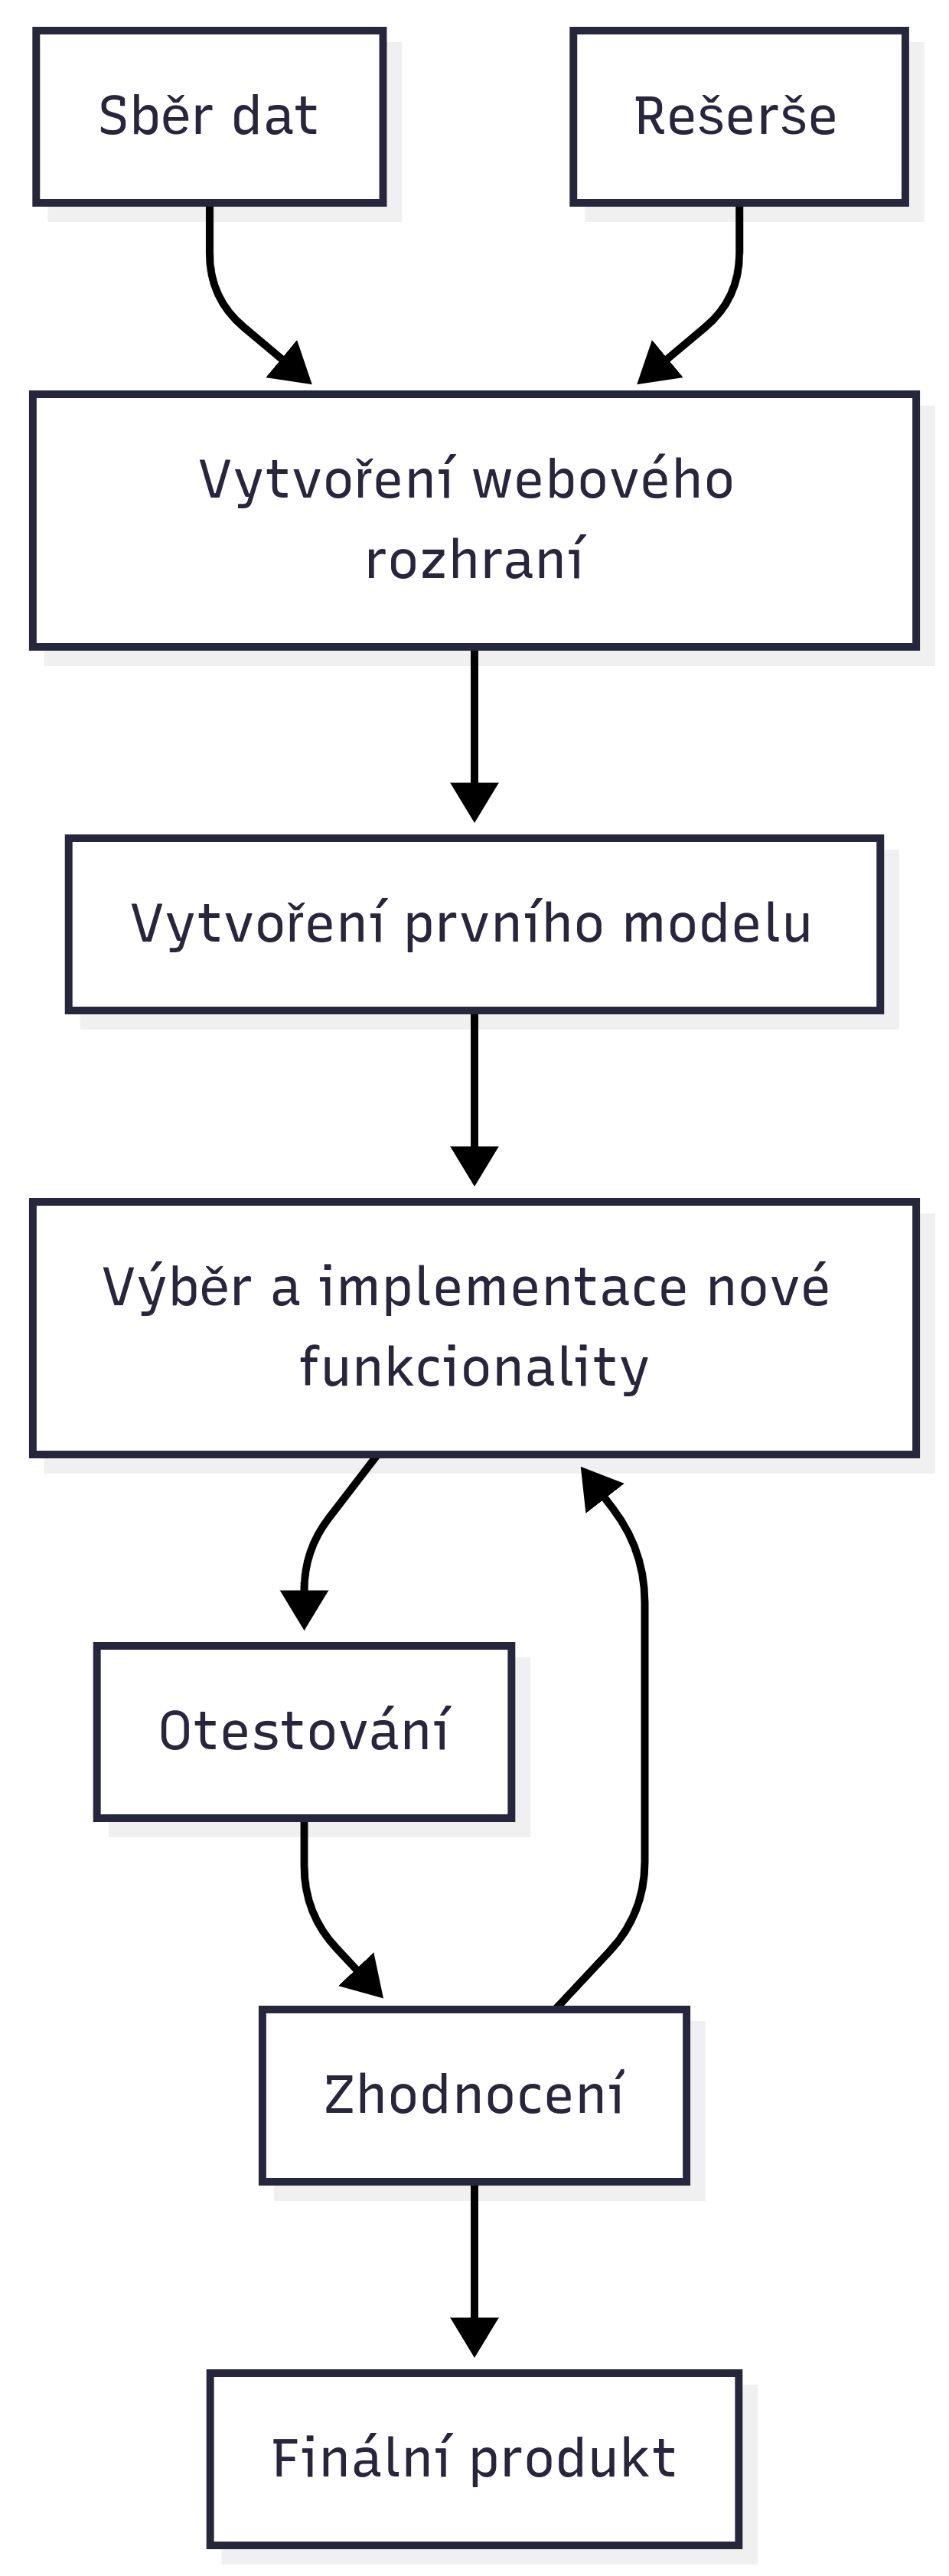
\includegraphics[height = 7.3cm]{flowchart.png}
  \end{center}
\end{frame}

\subsection{Tech-stack}
\begin{frame}{Tech-stack}
  \begin{itemize}
    \item Frontend
      \begin{itemize}
        \item Streamlit
        \item Python
      \end{itemize}
    \item Backend
      \begin{itemize}
        \item Python
        \item Knihovny: Yfinance, google\_news\_api, playwright, beautifulsoup, newspaper, pytorch, SQLalchemy, pymongo 
      \end{itemize}
    \item Databáze
      \begin{itemize}
        \item Opce: TimescaleDB (rozšíření PostgreSQL)
        \item Články (analýza sentimentu): MongoDB
      \end{itemize}
    \item Docker
  \end{itemize}
\end{frame}

\begin{frame}{Seznam literatury}
  \printbibliography
\end{frame}

\end{document}
